\documentclass{article}
\usepackage{graphicx} % Required for inserting images
\usepackage{float}
\usepackage{graphicx}
\usepackage{biblatex}
\addbibresource{report.bib}
\title{Minesweeper Cricket project report}
\author{Sanchana Arun }
\date{June 14 2023}

\begin{document}
\maketitle
\section{Introduction}
I chose Web coding as the topic for my assignment where we were asked to make a game which was a combination of Minesweeper and Cricket. I had made a total of 8 different tries in building this game before finalising one. Even though I had done 8 trials for this, I will be reporting 4 significant ones on here which includes the final project. I will walk you through all the changes my project underwent.
\maketitle
\section{Prototypes} Before we go into the trials, here is a small introduction about how I designed the game.
The first trial was a very basic one from which I started improvising. I chose the game to be a one player game which consists of a 6x6 grid that means there are 36 blocks in it. 11 fielders are randomised in these 36 blocks which on click, turns red and the game is over. When the player clicks on blocks which does not contain any fielders turns green which indicates you have earned one run. However, I have randomly added 10 bonus blocks which upon click turns purple and the score is raised by 6.
\maketitle
\subsection{Prototype 1}
The first time I worked on this project, I made it in a very basic manner, this one did not have any bonus blocks, and the game looked something like this:
\begin{figure}
[H]
   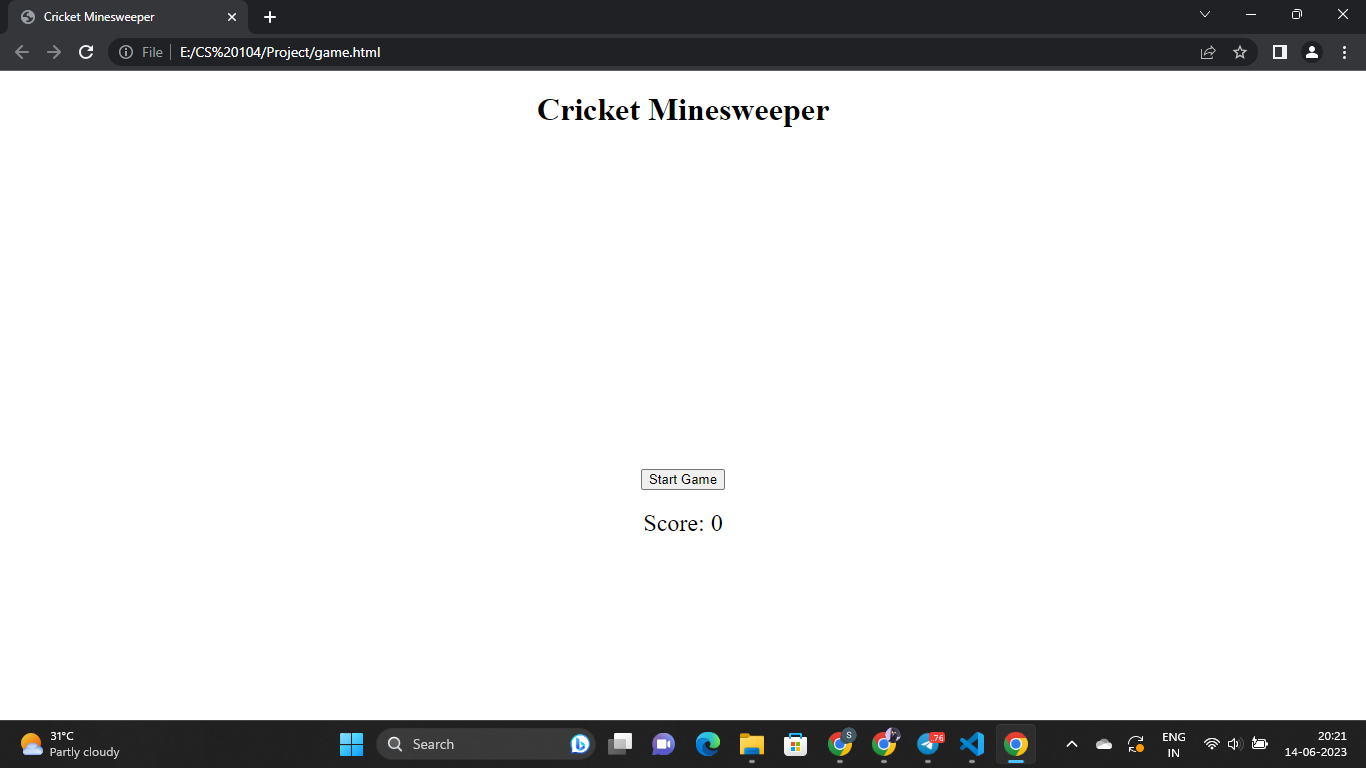
\includegraphics[width=\linewidth]{Screenshot (217).png}
   \caption{The first trial}
\end{figure}

After clicking on "Start Game":

\begin{figure}
[H]
   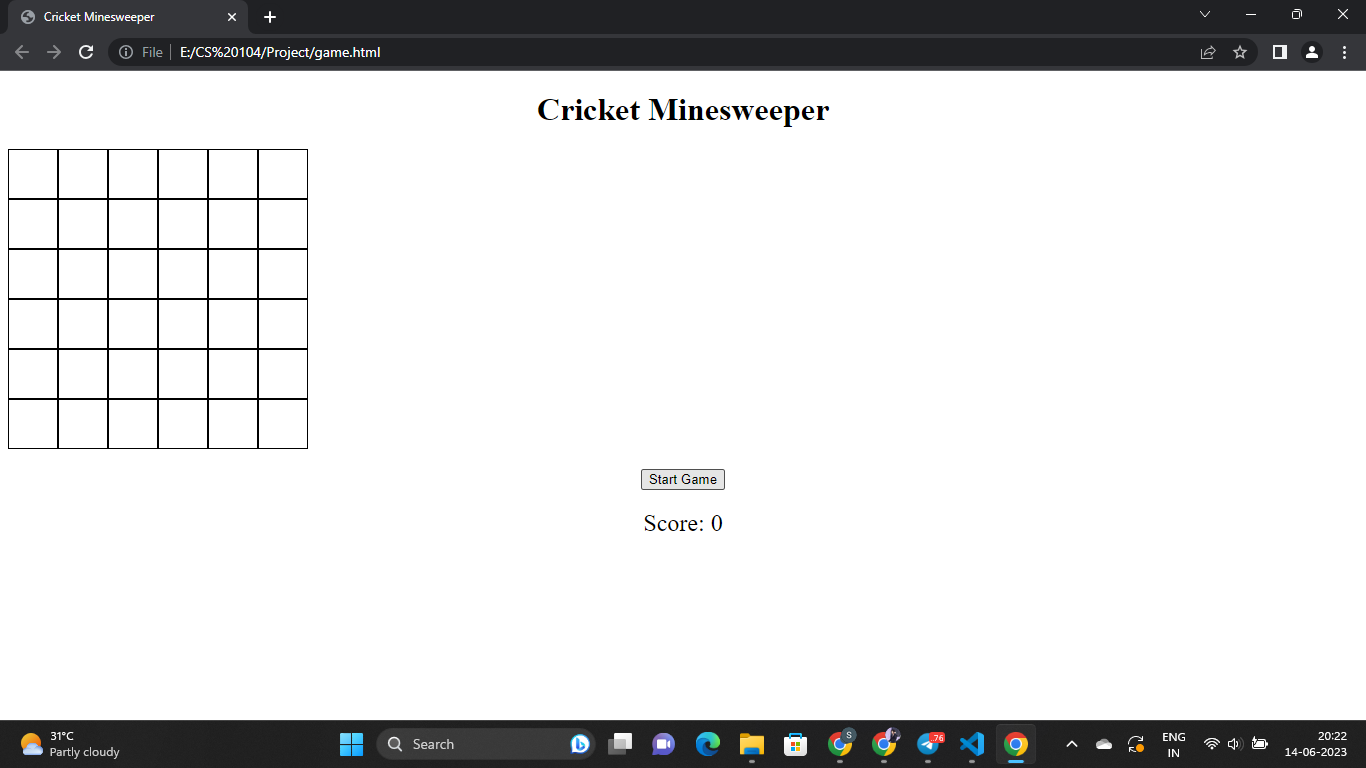
\includegraphics[width=\linewidth]{Screenshot (218).png}
   \caption{The Game Screen}
\end{figure}
\begin{figure}
[H]
   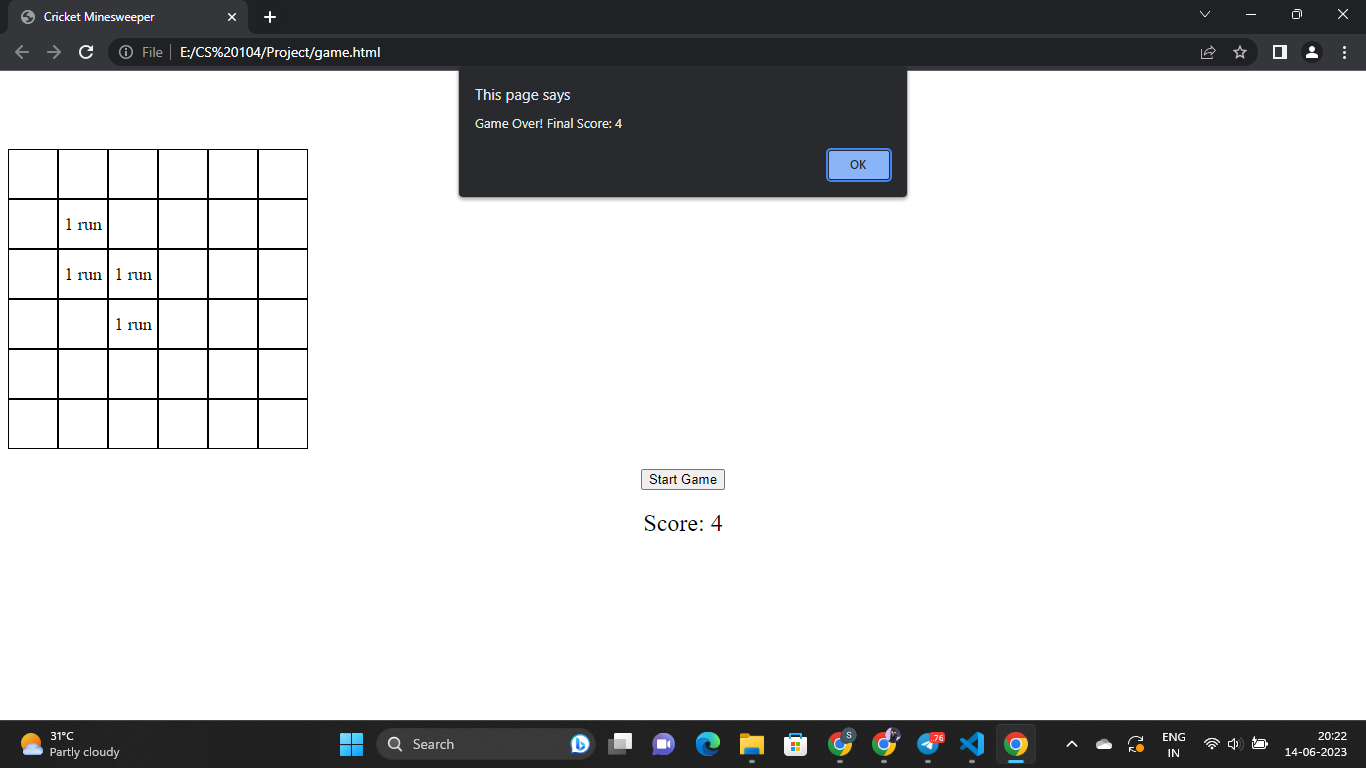
\includegraphics[width=\linewidth]{Screenshot (220).png}
   \caption{After playing the game}
\end{figure}

So this was basically the first prototype of this game.
\maketitle
\subsection{Prototype 2}
This one looks better than the first one with better interface. However I still have not added any bonus blocks or background image and it looked something like this:
\begin{figure}
[H]
   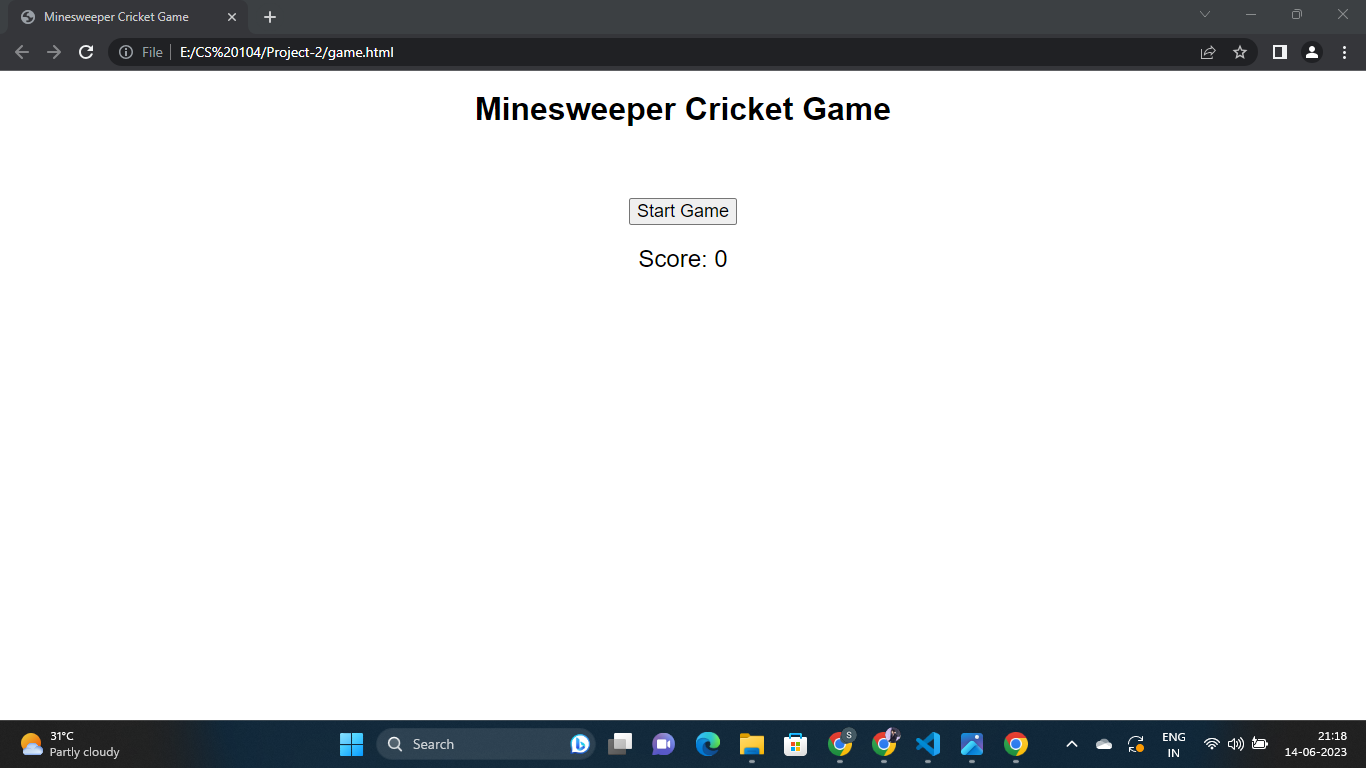
\includegraphics[width=\linewidth]{Screenshot (221).png}
   \caption{The second trial}
\end{figure}
After clicking on "Start Game"
\begin{figure}
[H]
   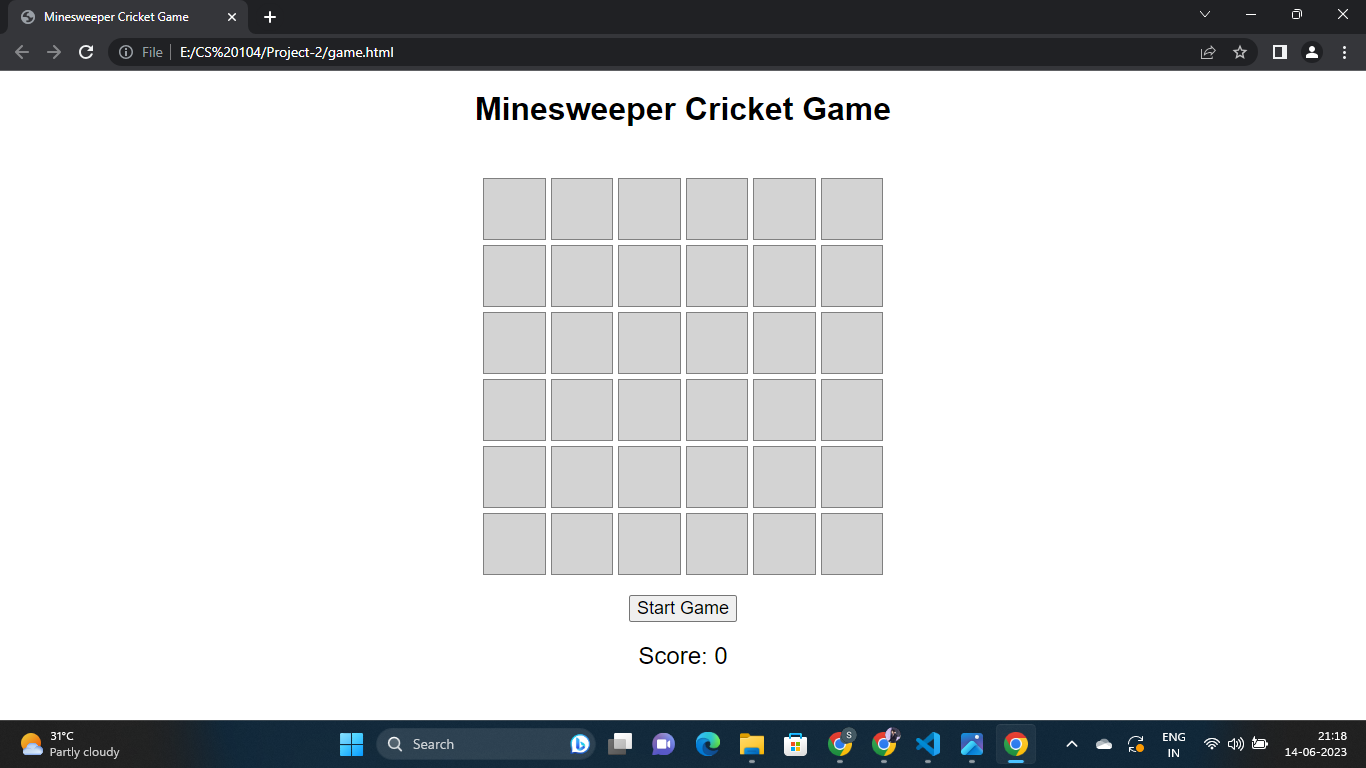
\includegraphics[width=\linewidth]{Screenshot (222).png}
   \caption{The game screen}
\end{figure}
\begin{figure}
[H]
   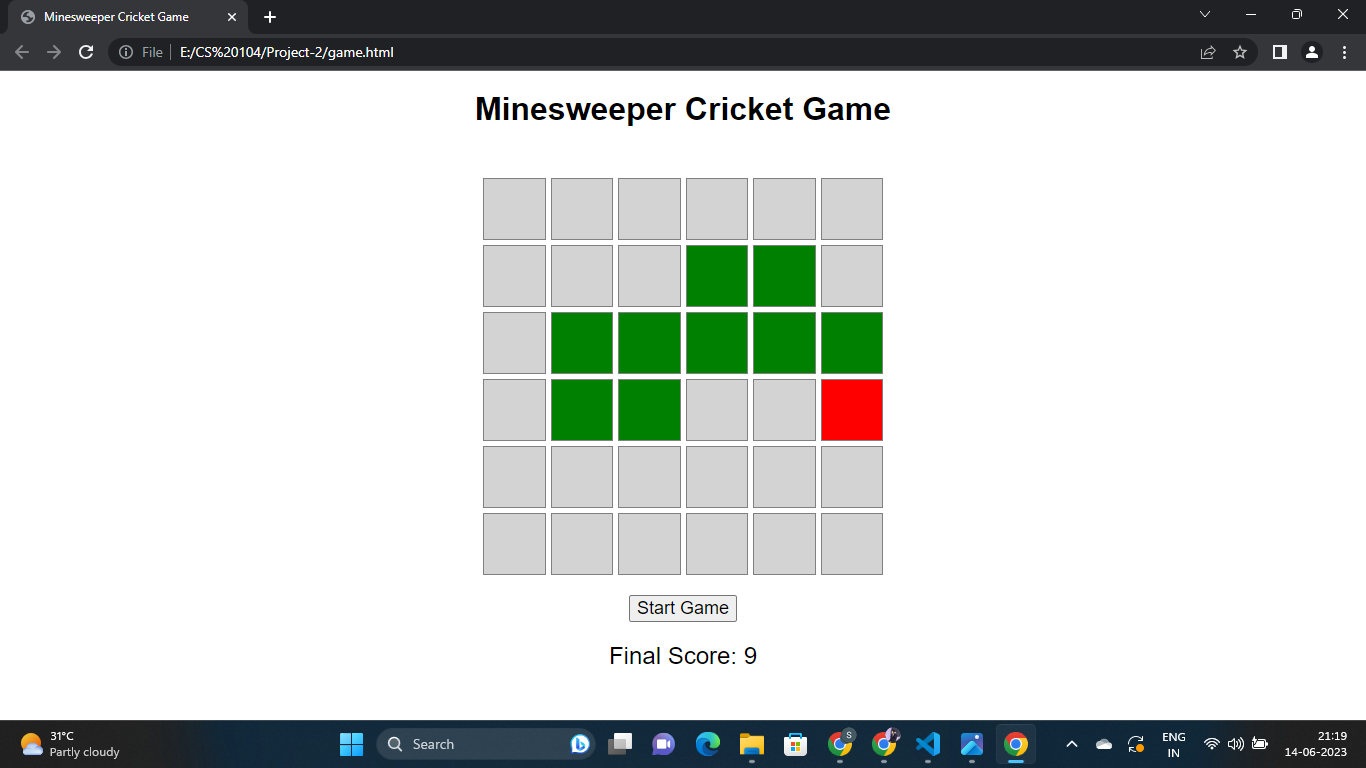
\includegraphics[width=\linewidth]{Screenshot (223).png}
   \caption{After playing the game}
\end{figure}
\maketitle
\subsection{Prototype 3}
Interface-wise, this one looked so much better than prototype 2. In this, I have randomised 10 bonus blocks among the 25 blocks remaining (11 fielders) which upon click turns the block purple and raises the score by 2. This one also did not have an appealing background. The background colour I chose here is beige (my favorite) I even made an attempt to make confetti fall at the end of the game but that didn't come off well so I dropped the idea. However I have added confetti in my final project. Prototype 3 looked something like this:
\begin{figure}
[H]
   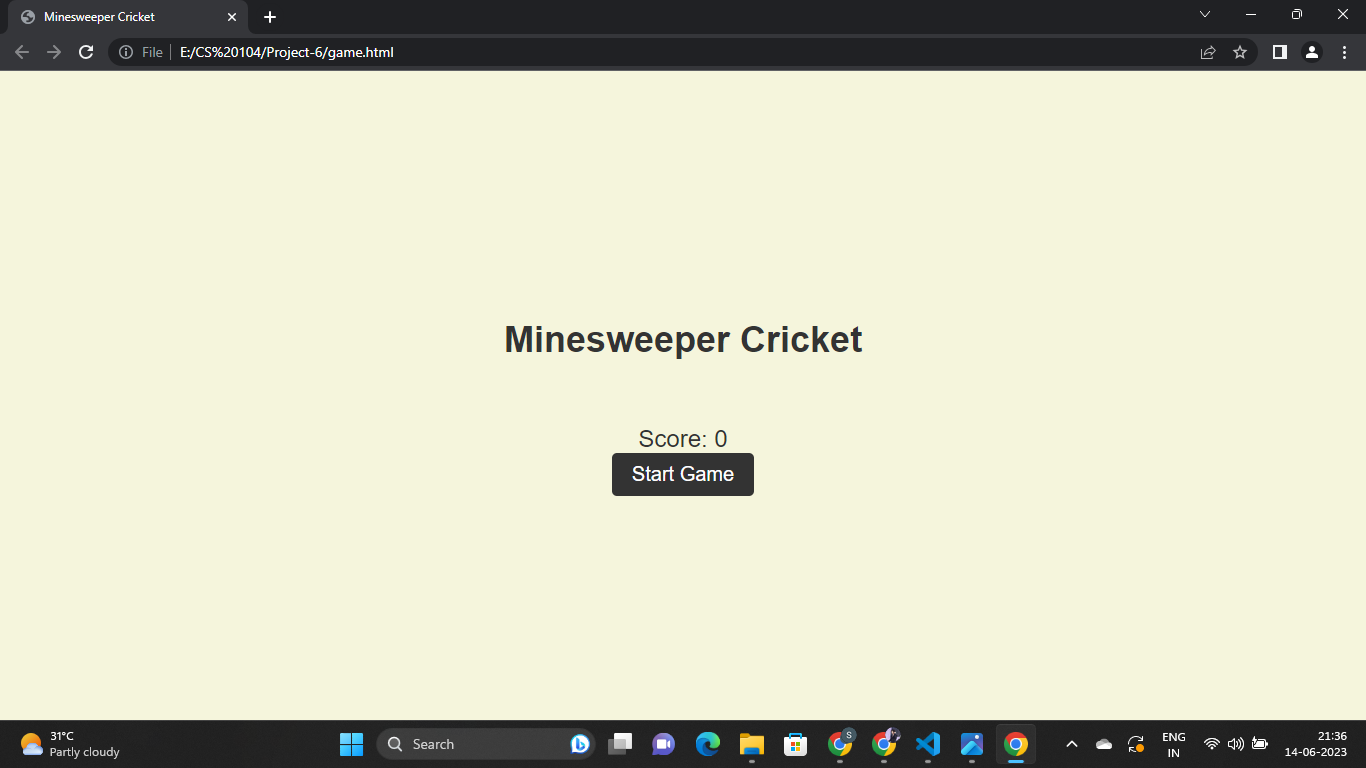
\includegraphics[width=\linewidth]{Screenshot (224).png}
   \caption{Trial 3}
\end{figure}
\begin{figure}
[H]
   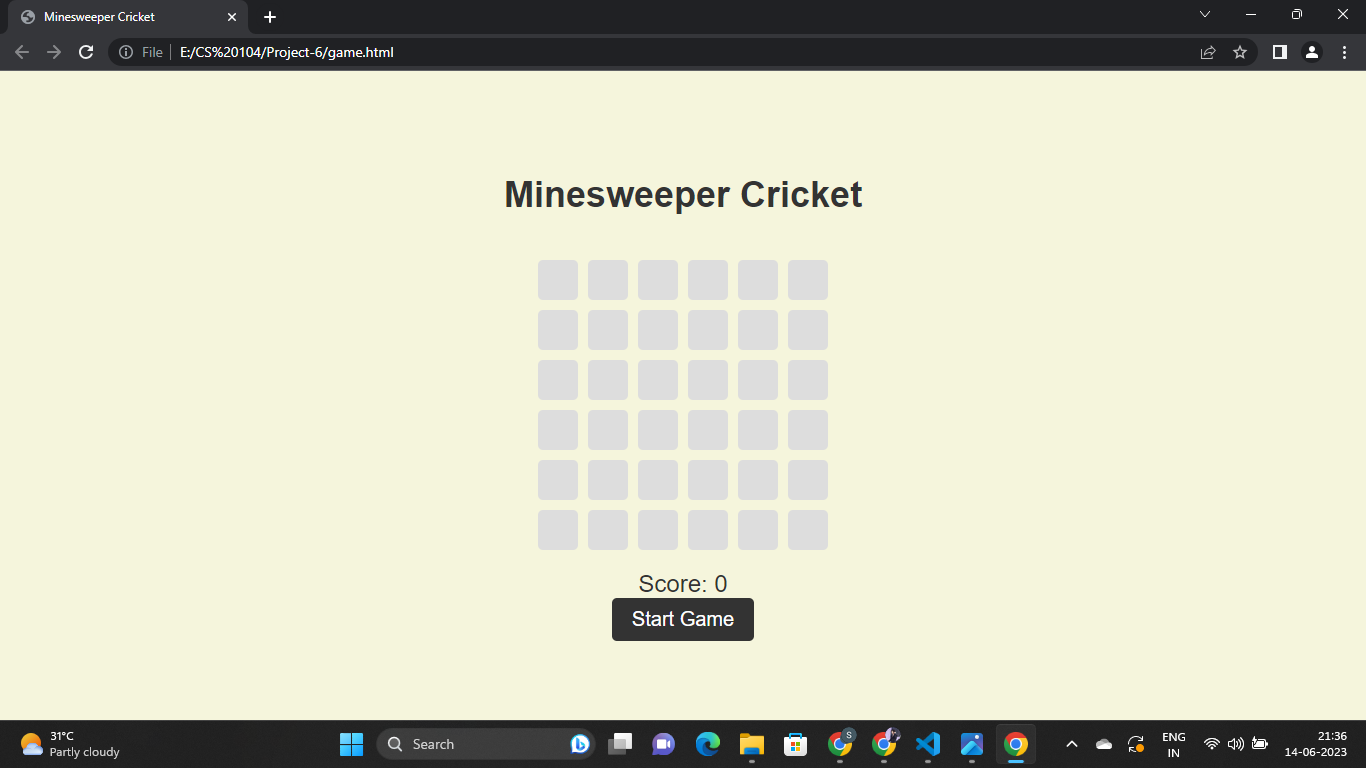
\includegraphics[width=\linewidth]{Screenshot (225).png}
   \caption{The game screen}
\end{figure}
As you can see, the prototype 3 looks much prettier and more like my final project. The purple block is a bonus block and it raises the score by 2.
\begin{figure}
[H]
   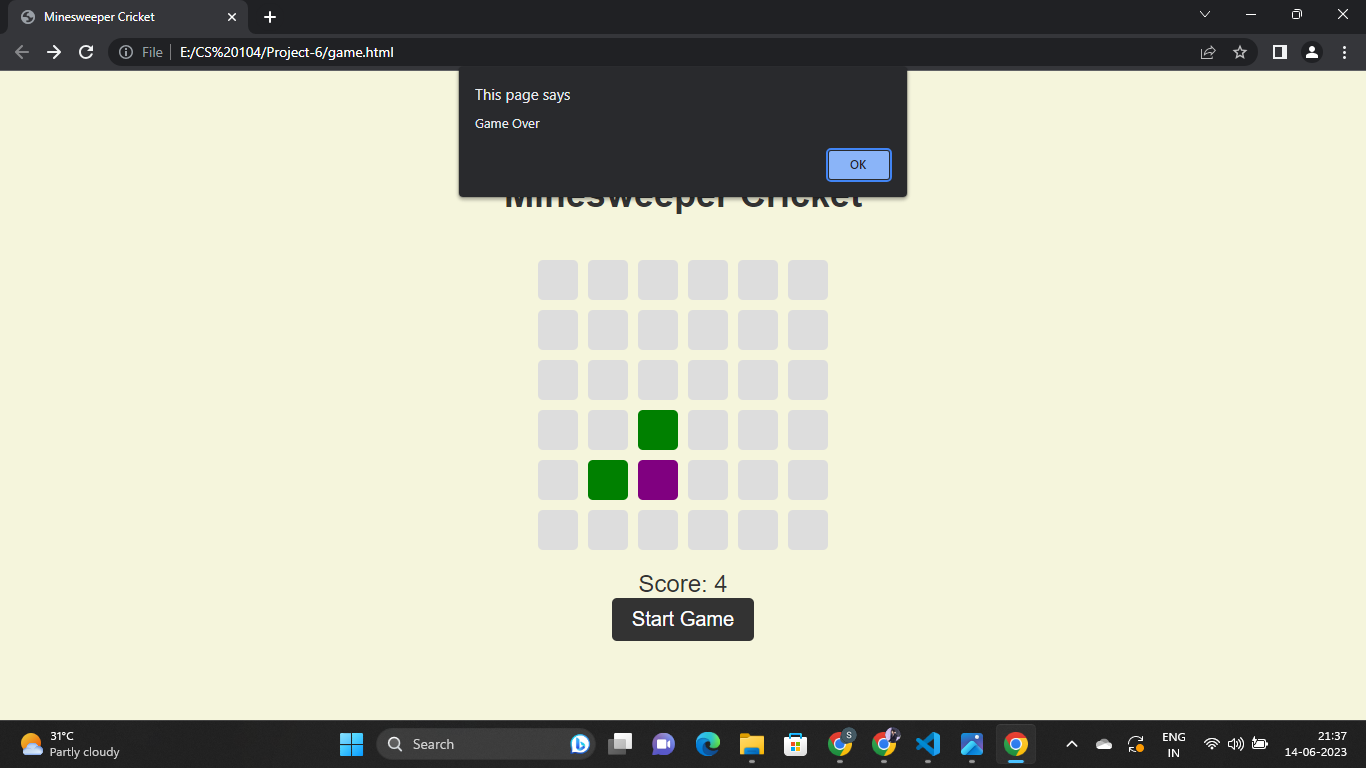
\includegraphics[width=\linewidth]{Screenshot (226).png}
   \caption{After playing the game}
\end{figure}
\maketitle
\section{The Final Project} In this, I changed the score raised upon clicking of purple block from 2 to 6. I created a pop us which says Game Over and asks if the player wants to continue playing and there are two buttons under it, one says 'Yes' and the other says 'No'. Once the player clicks 'Yes', the game will be initiated again and when the player clicks on 'No' the player is redirected another screen where there is a "Play Game" button and confetti falling. I have added AI generated background images in this project which makes it visually appealing. 
\begin{figure}
[H]
   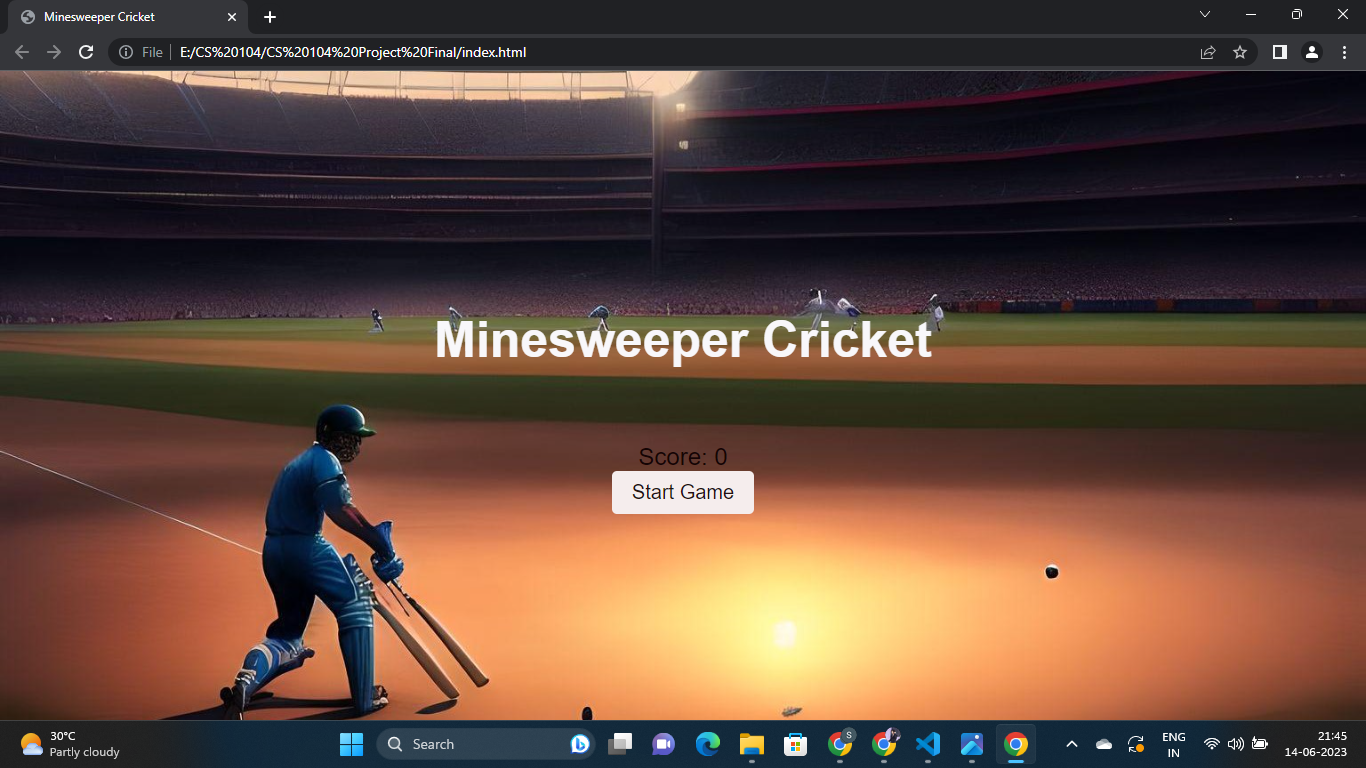
\includegraphics[width=\linewidth]{Screenshot (227).png}
   \caption{Final Project}
\end{figure}
\begin{figure}
[H]
   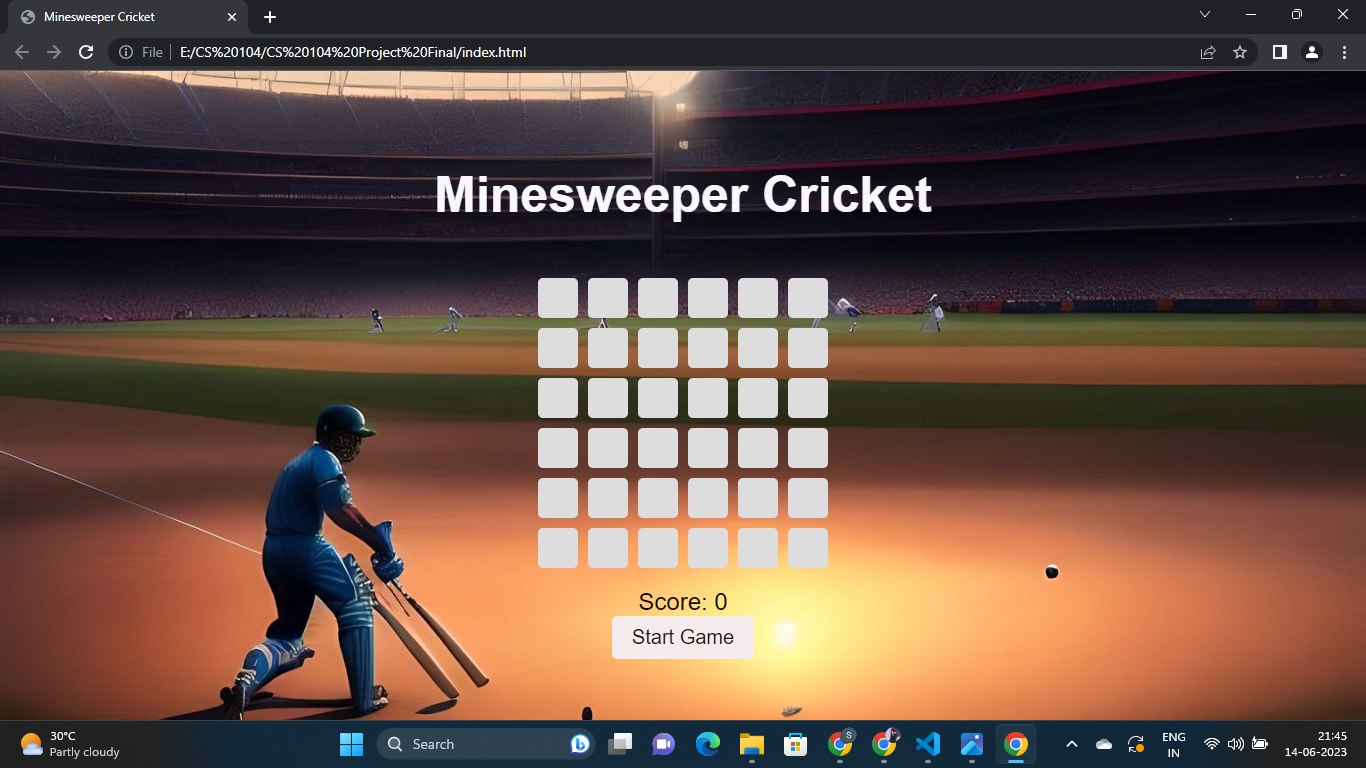
\includegraphics[width=\linewidth]{Screenshot (228).png}
   \caption{The game screen}
\end{figure}
\begin{figure}
[H]
   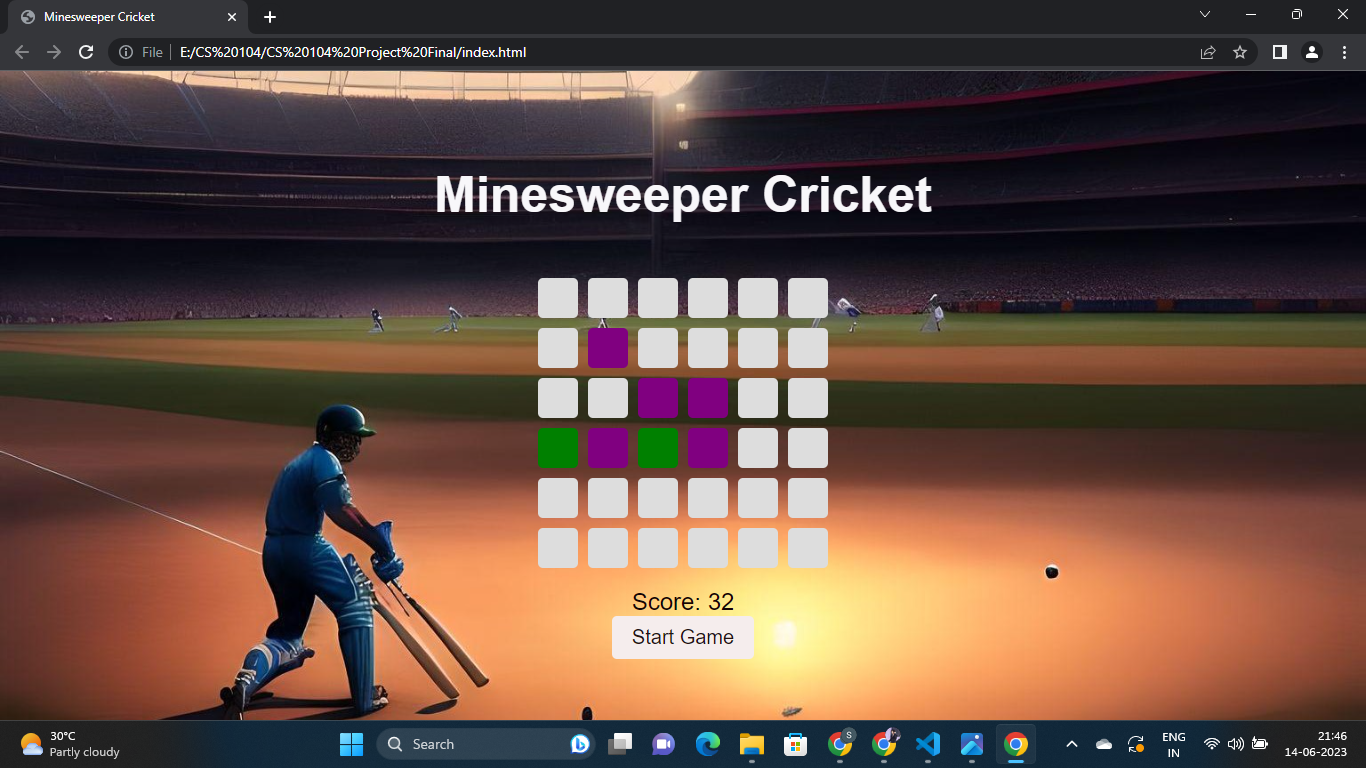
\includegraphics[width=\linewidth]{Screenshot (229).png}
   \caption{Green and Purple blocks}
\end{figure}
\begin{figure}
[H]
   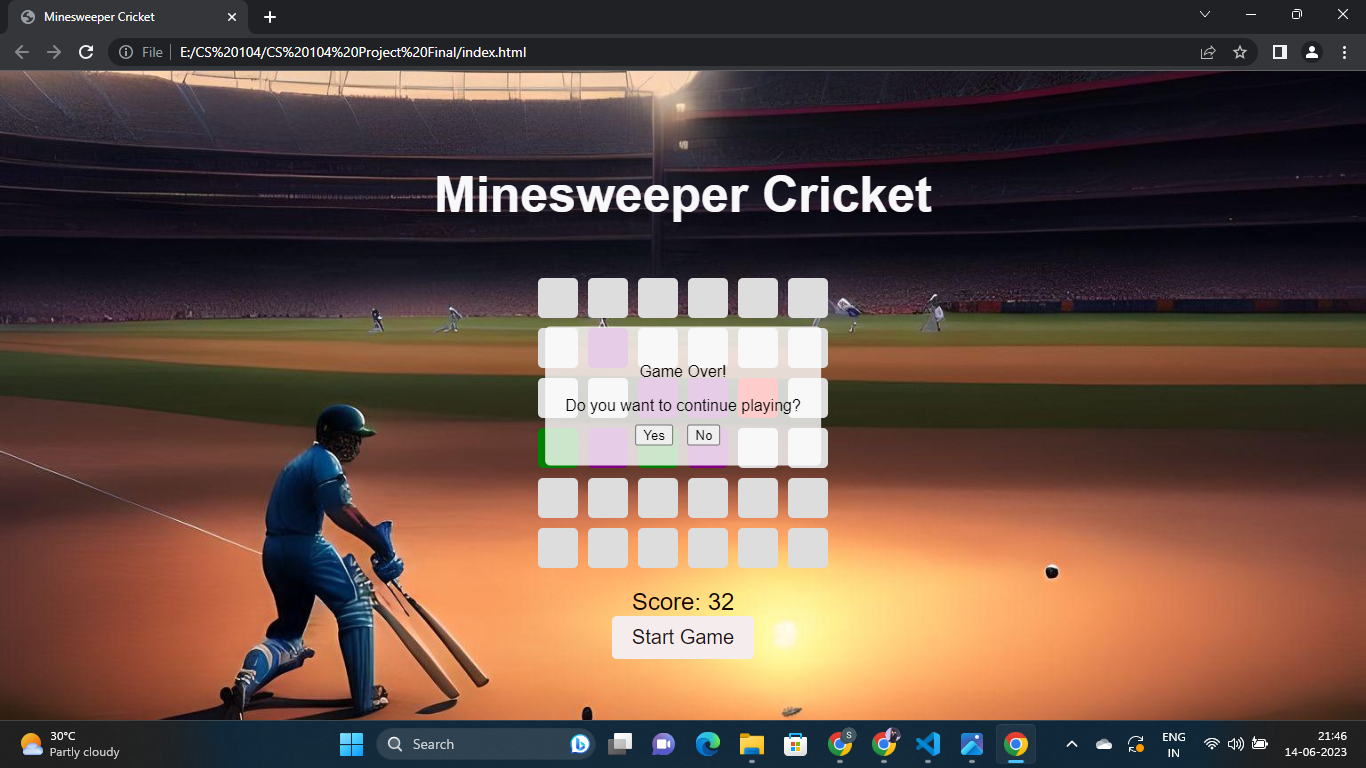
\includegraphics[width=\linewidth]{Screenshot (230).png}
   \caption{Game over and pop-up}
\end{figure}
\begin{figure}
[H]
   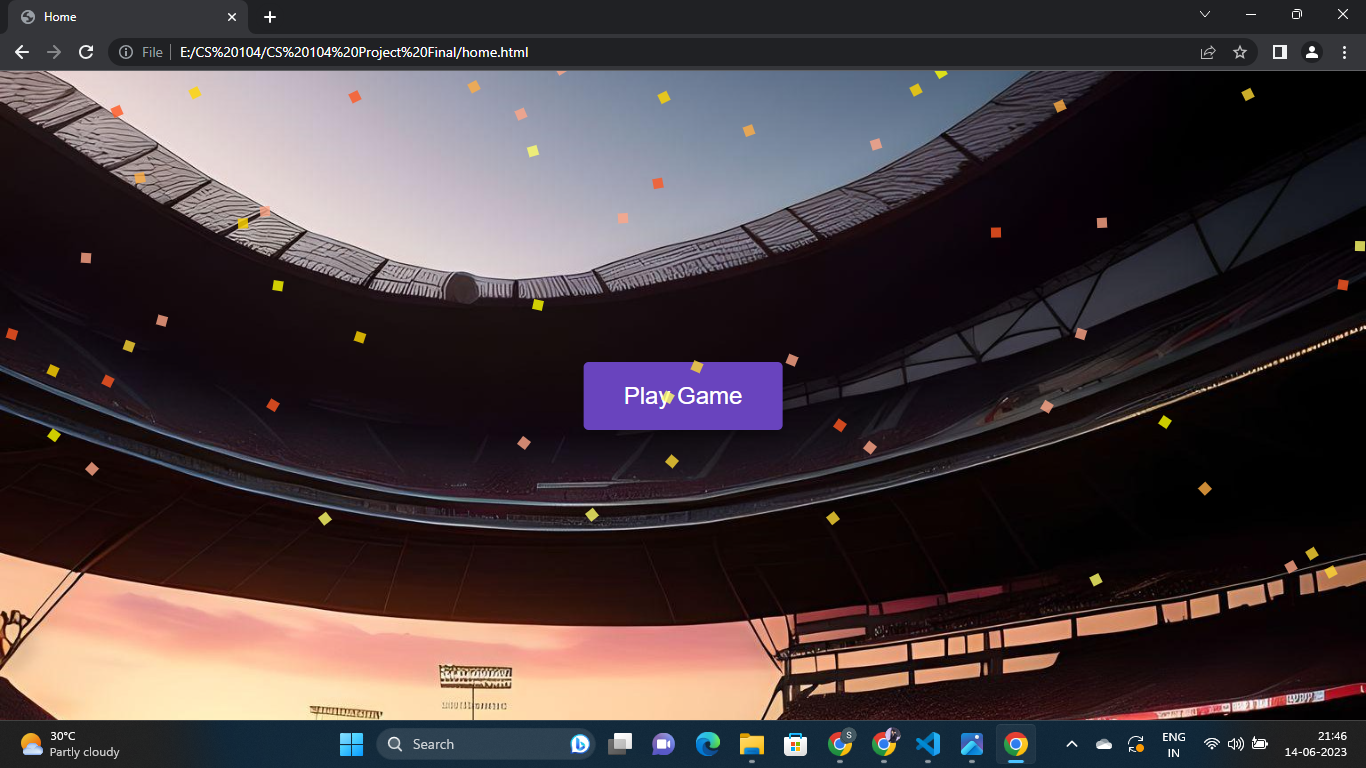
\includegraphics[width=\linewidth]{Screenshot (231).png}
   \caption{Redirected to another screen upon clicking 'No'}
\end{figure}
Upon clicking of 'Play Game' on the redirected screen, the game is directed to the home screen from where the player can choose to play the game over again.
This is all about my project. I hope you like it.
\nocite{*}
\printbibliography
\end{document}
